% This file should be built with
% xelatex, not the standard latexmk.

\documentclass[conference]{IEEEtran}
\IEEEoverridecommandlockouts
% The preceding line is only needed to identify funding in the first footnote. If that is unneeded, please comment it out.
\usepackage{cite}
\usepackage{amsmath,amssymb,amsfonts}
\usepackage{algorithmic}
\usepackage{graphicx}
\usepackage{textcomp}
\usepackage{xcolor}
\usepackage{multirow}
\usepackage{tabularx}

% Enable multilingual typesetting
\usepackage{polyglossia}      % Supports multiple languages and their configurations
\setdefaultlanguage{english}  % Set main language to English
\setotherlanguage{urdu}       % Add Urdu as a secondary language

% Font setup for each language
\newfontfamily\urdufont[Script=Arabic,Scale=2]{Jameel Noori Nastaleeq} % Urdu font                 % English font

\def\BibTeX{{\rm B\kern-.05em{\sc i\kern-.025em b}\kern-.08em
    T\kern-.1667em\lower.7ex\hbox{E}\kern-.125emX}}
\begin{document}

\title{UniversalPython - A Multilingual Python Programming Language*\\
{\footnotesize \textsuperscript{*}
Note: This draft was submitted in partial fulfillment of the requirements for the course "Research Methodology"
at FAST-NUCES

}
% \thanks{Identify applicable funding agency here. If none, delete this.}
}

\author{\IEEEauthorblockN{Saad Ahmed Bazaz}
\IEEEauthorblockA{\textit{Software Engineering and Product Design} \\
\textit{Grayhat}\\
Islamabad, Pakistan \\
bazaz@grayhat.studio}
}

\maketitle

\begin{abstract}
    % All widely used and useful programming languages have a common problem. They restrict entry on the basis of knowledge of the English language. The lack of knowledge of English poses a major hurdle to many newcomers who do not have the resources, in terms of time and money, to learn the language. Furthermore, studies back up the fact that learning is better when it’s done in the person’s local language. Therefore, we propose a language wrapper built on top of the Python programming language which can be directly used in the native Urdu language. This eliminates the need for any intermediate language as well. In the future, we aim to scale the language to encapsulate more languages to increase the availability of programming.
\end{abstract}

\begin{IEEEkeywords}
multilingual, programming language, internationalization, python, artificial intelligence, machine translation
\end{IEEEkeywords}

\section{Introduction}

% The first step to better understanding is communication. We use language to communicate concepts and produce thoughts. When teaching and educating, it is preferable to speak in the learner's native language to facilitate the understanding process.

% Computer science is a field dominated by the English language. Beginners must be acquainted with English to understand basic logical constructs. Without a real-life translator, learning programming concepts just by looking at English words is often impossible.

% Therefore, there is a need for formal translation of programming constructs into other languages and a usable framework for learners to program in their native language.

\section{Related Work}

High-level computer programming languages have been predominantly in the English language, ever since the first widespread high-level programming language, FORTRAN \cite{backus1978history}. It is interesting to note, however, that the first high-level programming language recorded in history, the “Plankalkül” of Konrad Zuse \cite{zuse1963ansaetze}, often considered a forerunner of today's programming languages \cite{bauer1972plankalkul}.

\subsection{Learning in your own language}
- Students in K-12 are able to learn better in their localized language. Start with general education, then with computer-related education.

  - https://unesdoc.unesco.org/ark:/48223/pf0000161121 \cite{buhmann2008mother}

  - Non-dominant languages \cite{taylor2015finding}
  
  - Learning to code in localized programming languages \cite{dasgupta2017learning}

  - A Framework for the Localization of Programming Languages \cite{swidan2023framework}

  - \cite{otten2023towards}

  ...

- There have been multiple attempts at non-english (needs a better term, maybe monolingual) programming languages (Russian, Kalaam \cite{Kalam_Programming_Language}, chronological order)
  - Issues?

- There have been multiple attempts at multilingual programming languages (Hedy \cite{Hermans_Hedy_A_Gradual}, chronological order)
  - Bigger Issues?

- There have been multiple attempts at localizing existing programming languages (PsueToPy, UrduScript \cite{Memon_UrduScript_2019}, Chinese Python)
  - Biggest Issues?
    - Scalability to different languages


% Studies have shown that students face problems learning the syntax and rules of a programming language initially [1]. However, learning in a local language has a significant positive impact on learning outcomes [2]. This supports the idea that programming should not be restricted by a language barrier.

\subsection{Multilingual/Localized Programming Languages}

PsueToPy \cite{IEEEexample:tamethebeast} proposes an intermediate pseudo language to communicate with the Python interpreter. This approach adds complexity for users due to potential inconsistencies in machine translation. Additionally, PsueToPy lacks a standard structure, making it difficult to transition between languages. 

An African-based programming language [5] faced scalability issues and a lack of community backing. Another approach involved editing the Python source code to accommodate Chinese symbols [6]. However, this method is difficult to implement and maintain across different versions and languages.

Several attempts have been made to create Urdu programming languages [7, 8, 9, 10]. However, they suffer from issues like using Roman Urdu instead of Arabic script, lacking open-source libraries, and limited scalability to other languages.

UrduScript [7] is similar to our approach but uses JavaScript instead of Python and Roman Urdu script. Our method leverages Python's extensive libraries and utilizes the more familiar Arabic script for Urdu speakers.

\subsection{Multilingual Programming Environments}

Approaches have been made to address the issue of development environments not supporting multiple languages [11, 12]. Additionally, some work translates Python programs into traditional Chinese for explanations [13]. However, this method uses Google Translate, making it slow and unsuitable for programming purposes.

Our framework allows easy support for UniversalPython plugins in existing Python IDEs. It acts as a bridge, translating Urdu code into English before passing it to the IDE.

\section{Design of UniversalPython}

We propose a framework as shown in “Fig. 1“, which is a wrapper around the Python Engine. The user writes code in Urdu, for example:

\begin{figure}[htbp]
\centerline{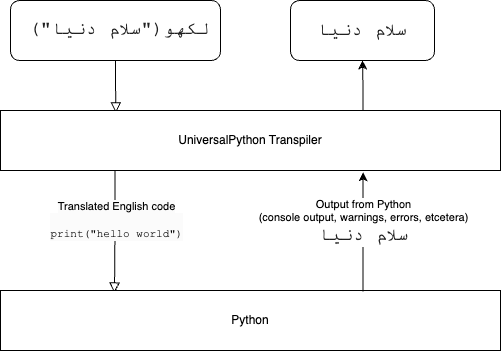
\includegraphics[width=\columnwidth]{UniversalPython-flowchart.png}}
\caption{A high-level abstraction of how the UniversalPython transpiler works.}
\label{fig}
\end{figure}

Throughout this paper, we take the example of **Urdu**, the national language of Pakistan, and a traditional Right-to-left language, as a translation language. 

The user writes code in Urdu, for example:




This is passed to “UniversalPython”, which first translates the code to English using Lexical Analysis and Parsing with the PLY library.
To do this, it first loads the Urdu dictionary, which is a YAML file containing mappings from Urdu to English. This dictionary is a mapping of each Urdu word to a Python keyword. Here is an example of such a dictionary:
In PLY, we have the option to reserve some keywords so that the library automatically tokenizes them. We set a Grammar Rule which, whenever a reserved keyword (i.e. a word which is present as a key in a language dictionary) is tokenized, simply looks for the token in the language dictionary (key) and replaces it with the corresponding English keyword (value).
We also set a Grammar Rule to ignore all content within double quotes or single quotes (i.e. strings and docstring) and to ignore content in comments (which start with a \#). We achieve this using Regular Expressions.
Urdu numbers also lie on the Unicode scale. ۰ (or roman 0) is at 1776, while ۹ (or roman 9) is at 1785.

Keeping this in mind, we define a Regular Expression which detects any symbols equal to or between this range, 1776 - 1785. These are the Urdu digits. We then use the same language dictionary to translate these numbers into roman numerals. For example, ۵ becomes 5, ۹۰ becomes 90, ۱۰ becomes 10, ۲۰۲۲ becomes 2022.
Furthermore, we also replace all periods ( . ) and commas ( , ), as these look different in Urdu than they do in English.

The rest of the code remains untouched. Whether it is a symbol,like :, ( or ), etc, or even if it causes the lexer to crash, we ignore it so we can preserve the original structure of the code as much as possible. It is not required to translate such symbols and errors anyway: They are meant to be handled by Python, not UniversalPython. Back to our initial example code, our engine detects and replaces it with print , 􏰁􏰃 is replaced with if ,
is replaced with else , and all Arabic digits are replaced with Roman digits. Hence the translated code would be:

The above code is essentially vanilla Python code which can now simply be executed by the Python engine. The Urdu variable name 􏰀 does not present any issue to Python, as from Python 3.0 onwards, Unicode is fully supported. So the above code is passed on to the Python engine. The Python engine outputs some response; it can be some print statements which the user entered, compiler/interpreter warnings, and/or errors. This response is passed up to UniversalPython, where again it is tokenized to replace keywords in case of error messages. In our example, since there are no errors, it simply outputs the response as-is. So the response would be:

To demonstrate the ease by which plugins can be made for UniversalPython, we made a wrapper for the IPython kernel in which we imported UniversalPython as a package, and processed the code (i.e. translated it from Urdu to English) before it was passed onto IPython. This way, we overrode the functions and achieved a working kernel for UniversalPython. It works line-by-line while maintaining the program memory. This also gave us a visual interface for the language to test it thoroughly.

The Urdu dictionary is a YAML file containing mappings from Urdu to English keywords, is used for translation. The PLY library allows reserving keywords for automatic tokenization and replacement with their English equivalents. Additionally, grammar rules are set to ignore content within quotes, comments, and Urdu numbers (which lie on the Unicode scale).

\section{Experimentation}

\subsection{Evaluation metrics}\label{AA}

We propose the following metrics which UniversalPython should meet in order than it is considered effective:

1) Programs which work in Python, should be recreatable in UniversalPython, and vice versa.

2) UniversalPython should operate as a reasonable speed which at least does not disturb the programmer.

3) UniversalPython should be able to translate from one non-English language to another

4) A benchmark should be made against other existing multilingual and non-English monolingual languages

5) A user experience test should be conducted to find out user acceptability towards a language in their native tongue.

\subsection{Benchmarks with Python}\label{BB}

Time: Check the execution time / performance of Python vs UniversalPython. We use a benchmarking tool called hyperfine which runs each program multiple times to produce a mean execution time.

Conversion: Convert simple programs from English Python to UniversalPython, and test if they still work. Our testing mechanism for the above is as below:
1) We take an existing Python program, lets say multiplication.py.
2) Run the UniversalPython system in reverse. This will flip the language dictionary and generate an Urdu version of the program (all the keywords would be translated from English to Urdu). Save it as multiplication.ur.py.
3) Run multiplication.ur.py using UniversalPython, and multiplication.py using Python. If both give the same output on the terminal then no data loss has occurred; Both Urdu program and English program output the same message. Hence we can say that the program has safely converted from English to UniversalPython and vice versa without breaking the code or changing the logic.

We take simple algorithmic programs from TheAlgorithms/Python [14], a repository containing implementations of well-known algorithms, in the Python programming language. We run a loop over them and run the above algorithm on each to test.

\section{Results}

We evaluate the results of the experiment mentioned above in the following two ways:
Execution Success Rate After running the experiment, we were able to achieve the following results.

“Table III“ describes our results over 110 simple Python programs present in TheAlgorithms/Python [14] maths implementation.
We reported that 98\% of simple programs can be automatically converted into Urdu Python without breaking the code. Amongst the programs that failed, the reason was due to a problem in generating the Urdu version of an English program (i.e. running Urdu Python in reverse) - it cannot distinguish between “is” and “==”, as they have the same purpose in English Python.
Execution Time Upon recording the execution time summary of the experiment we concluded that Urdu Python performed better with simpler and less wordy pro- grams, whereas for more wordy and lengthy algorithms, python performed better in terms of execution time. How- ever, it is well within the range of acceptable speed of a programming language. Some of the top differences in performances of some algorithms can be seen in the tables “Table IV“ and “Table V“.
Table IV: Execution times of functions where our engine performed well.

It is possible to make this framework generic \textit{enough} to span multiple languages. We managed to make three variants; Urdu, Chinese and Hindi, to demonstrate UniversalPython's capability to extend multiple languages.

\section{Limitations}

- Third-party library support is vital for any software platform to flourish. While third-party libraries do not cause the program to crash, we would prefer a better developer experience in which third-party libraries are also translated.

- It is currently not possible translate words with spaces in between them. For example, `elif` in Python actually translates to ورنہ اگر in the Urdu language. Some languages may also have different placements for verbs and nouns, and different words for different quantities (e.g. mono, bi, tri). This may present a challenge for UniversalPython, where more creative effort may be needed to construct a better front-end experience for programmers, while ensuring compatibility with Python.

- In order to increase the accuracy of the translations, a translation-verification system can be developed, where beginner and experienced programmers can be asked, "How would you write the following snippet of code in your language?", and let them write the code in any shape or form they desire. This could be done with data from platforms like Leetcode, however, we leave that to the imagination of the reader.


\section{Future Work}

UniversalPython can be developed as an extensible programming language which would grow alongside Python and would be interoperable with it. It is also maintainable, because since it is simply a wrapper, only the keywords need to be updated in the dictionary, and it will work for any future (or past) versions of Python. Furthermore, it is scalable to other languages because the dictionary structure allows for any language to be added to UniversalPython.

To improve the current implementation, it would be useful to accommodate as many Python keywords as possible, preferably all of them. It would also be useful to separately have translations for major libraries/packages such as pandas, numpy, cv2, etc. A scalable and efficient method for this would be to automatically scan such libraries(the Python source code) to identify important keywords, automatically translate them to the nearest and best possible Urdu word, and add them to the Grammar. This can be achieved using Natural Language Processing, Deep Learning, Machine Learning and similar methods.

In the current framework, making it possible for the user to choose whether or not to detect variables and functions, and machine-translate them into their corresponding names, could make the experience better.

It would also be helpful to conduct User Experience tests for UniversalPython, so that it can be determined whether or not UniversalPython really does benefit people who speak Urdu to learn programming.

Designing and developing a better test metric to test the effectiveness of such a framework would also be useful for UniversalPython.

\section*{Acknowledgment}

I would like to acknowledge my mentor, Dr Omer Beg, for always guiding me to the right path during my Bachelor's, professional life, and Master's degree.

\bibliographystyle{bibtex/IEEEtran} % Or your desired style (e.g., IEEEtran)
\bibliography{bibtex/IEEEexample} 

\vspace{12pt}
\end{document}
